\documentclass{subfiles}

\begin{document}
    Zuerst kann man das verlauf des Potentials $V(x,y)$ zeichnen. Hier ist $m_{E}$ = 10 \cdot $m_{M}$.
    \begin{figure}[H]
        \centering
        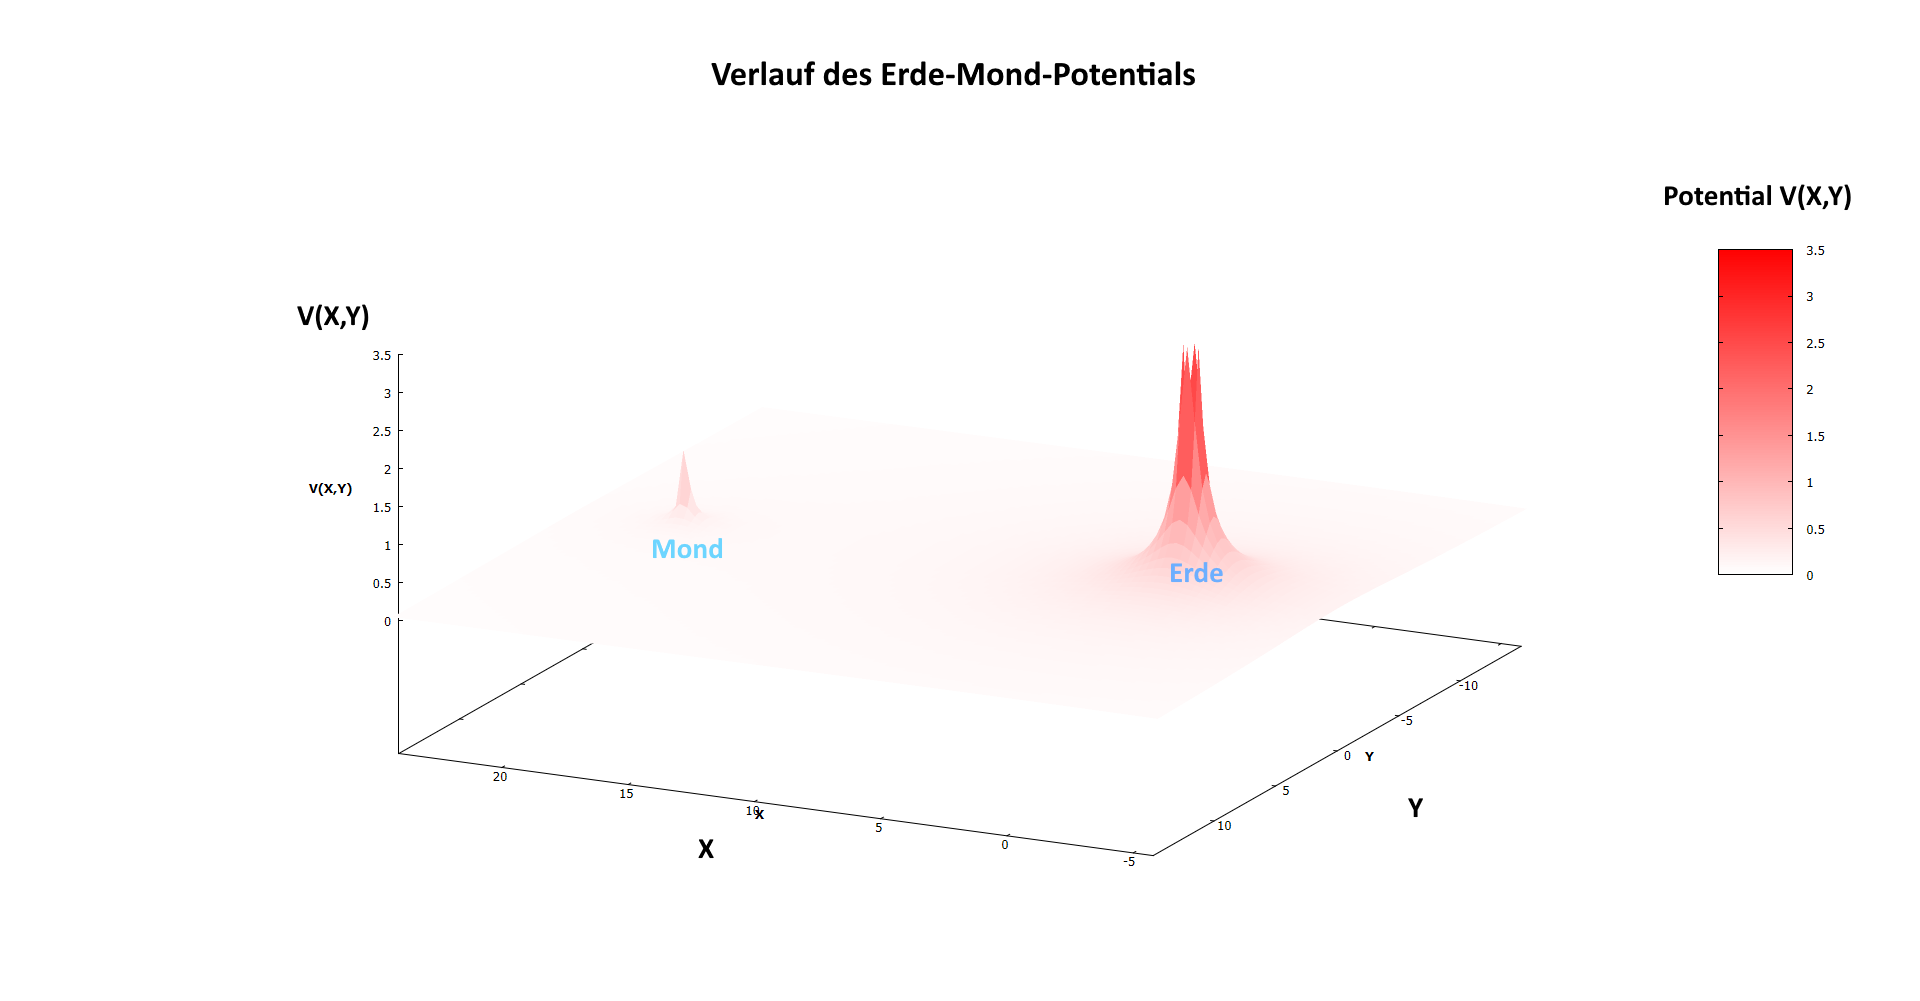
\includegraphics[width=0.8\textwidth]{../Ressource/PotentialVerlauf.png}
        \caption{Potentialverlauf}
        \label{fig:Potential}
    \end{figure}
    Für praktische Gründen sind die Abstände zwischen die Planetten viel kleiner. Hier sollte die Größenordnung $\num{e9}$m sein.\\
\end{document}